\documentclass[12pt]{report}
\usepackage{graphicx} % Required for inserting images
\usepackage{setspace}
\usepackage[a4paper,top=2.8cm,bottom=2.8cm,left=3cm,right=3cm,marginparwidth=1.75cm]{geometry}
\usepackage{lipsum}
\usepackage[style=apa,backend=biber]{biblatex}
\usepackage{sectsty}
\usepackage{nicematrix}
\usepackage{adjustbox}
\usepackage{rotating, float, caption}
\usepackage{enumitem}
\usepackage{nomencl}
\usepackage{placeins}

\title{Examining the Viability of Net-Negative Carbon Removal Techniques: An Economic and Environmental Evaluation}
\author{Thimo Merke}
\date{June 15, 2023}

\usepackage{etoolbox}
\makeatletter
\patchcmd{\@makechapterhead}{50\p@}{0pt}{}{}
\patchcmd{\@makeschapterhead}{50\p@}{0pt}{}{}
\makeatother

\newcommand{\mychapter}[2]{
    \setcounter{chapter}{#1}
    \setcounter{section}{0}
    \chapter*{#2}
    \addcontentsline{toc}{chapter}{#2}
}

\onehalfspacing
\chapterfont{\fontsize{30}{15}\selectfont}
\sectionfont{\fontsize{14}{15}\selectfont}
\subsectionfont{\fontsize{12}{15}\selectfont}

\addbibresource{references.bib}

\begin{document}

\begin{titlepage}
\newcommand{\HRule}{\rule{\linewidth}{0.5mm}} % Defines a new command for the horizontal lines, change thickness here

%----------------------------------------------------------------------------------------
%	LOGO SECTION
%----------------------------------------------------------------------------------------
\center % Center everything on the page
\begin{figure}
  \centering
  \begin{minipage}[b]{0.4\textwidth}
    
\includegraphics[width=6cm]{figures/mises.jpg}
  \end{minipage}
  \hfill
  \begin{minipage}[b]{0.4\textwidth}
    
\includegraphics[width=6cm]{figures/uoma.jpg}
  \end{minipage}
\end{figure}
\vspace*{6\baselineskip}
%----------------------------------------------------------------------------------------

%----------------------------------------------------------------------------------------
%	TITLE SECTION
%----------------------------------------------------------------------------------------
\makeatletter
{\large \bfseries \@title}\\[0.4cm] % Title of your document
\vspace*{4\baselineskip}
%----------------------------------------------------------------------------------------
%	AUTHOR SECTION
%----------------------------------------------------------------------------------------
\begin{center} %\large
\textbf{Thimo Merke}\\  %Enter the name of the authors here
Student ID: 1566894\\
E-Mail: thmerke@mail.uni-mannheim.de\\
Address: Hessische Str. 54, D-68305 Mannheim, Germany\\
\vspace*{4\baselineskip} 
15.06.2023 \\
Supervisor: Philip Holler
\end{center}

\makeatother
\vfill % Fill the rest of the page with whitespace
\end{titlepage}

\begin{abstract}
This thesis examines the economic and environmental viability of carbon removal strategies as a means of mitigating climate change. It provides an overview of the current state of global greenhouse gas emissions and carbon removal efforts. It then explores various carbon removal strategies and analyzes economic and environmental factors affecting their feasibility, as well as their potential co-benefits and adverse side effects. The analysis finds that while some carbon removal strategies are more cost-effective at present, all have the potential to play a role in mitigating climate change. However, careful consideration must be given to the potential side effects of these strategies, particularly in terms of land use changes and ecosystem disruption. Based on the results, the thesis also provides recommendations for implementing carbon removal strategies. Ultimately, carbon removal cannot replace the urgent need for reductions in CO\textsubscript{2} emissions, but it can complement such efforts.
\end{abstract}

\tableofcontents
%\thispagestyle{empty}
\listoffigures
\listoftables
\newpage

\makenomenclature
\setlength{\nomlabelwidth}{.20\hsize}
\renewcommand{\nomlabel}[1]{#1 \dotfill}
\renewcommand{\nomname}{List of Acronyms}
\nomenclature{CDR}{Carbon dioxide removal}
\nomenclature{IPCC}{Intergovernmental Panel on Climate Change}
\nomenclature{NET}{Negative emissions technology}
\nomenclature{NAS}{National Academies of Sciences, Engineering, and Medicine (USA)}
\nomenclature{EU-ETS}{European Emissions Trading System}
\nomenclature{AFRF}{Afforestation and reforestation}
\nomenclature{EW}{Enhanced weathering}
\nomenclature{BCP}{Biological carbon pump}
\nomenclature{OF}{Ocean fertilization}
\nomenclature{OIF}{Ocean iron fertilization}
\nomenclature{OMF}{Ocean macronutrient fertilization}
\nomenclature{LNLC}{Low-nutrient, low-chlorophyll}
\nomenclature{HNLC}{High-nutrient, low-chlorophyll}
\nomenclature{DAC}{Direct air capture}
\nomenclature{LDAC}{Liquid solvent-based direct air capture}
\nomenclature{SDAC}{Solid sorbent-based direct air capture}
\nomenclature{BECCS}{Bioenergy with carbon capture and storage}
\nomenclature{MSW}{Municipal solid waste}
\nomenclature{CCS}{Carbon capture and storage}
\nomenclature{GHG}{Greenhouse gas}
\printnomenclature
\newpage

%\mychapter{0}{Introduction}
Earth has been going through cycles of cold periods ("glacials") and warm periods ("interglacials") for at least the last one million years. However, since the beginning of the industrial revolution in the mid to late 18th century, an increasing amount of anthropogenic CO\textsubscript{2} emissions has impacted the natural carbon cycle. While slight more than half of the total emissions since 1850 have been absorbed by land and oceans, the remainder has accumulated in the atmosphere \parencite{Bergman2021TheJustice} and increased the greenhouse effect, causing the atmosphere to warm up and resulting in serious and at least partially irreversible damage to terrestrial and ocean ecosystems and both human and animal life \parencite[9]{IPCC2022SummaryPolicymakers}. Currently, anthropogenic emission amount to about 40 billion tons of CO\textsubscript{2} globally every year \parencite[4]{Friedlingstein2022Global2022}, caused by energy generation, but also agriculture, construction, and transportation. Despite the ongoing and increasing efforts and pledges to curb carbon emissions by transitioning to green, or net-zero, technologies, we are currently on track for a global average temperature increase of 2.8 degrees Celsius by the year 2100, according to estimates of the \textit{United Nations Environment Programme}. With the successful implementation of all current carbon emission reduction pledges, global warming could be limited to 2.4 degrees Celsius, but this is still well above the 1.5-degree goal set in the \textit{Paris Agreement} that needs to be achieved to limit the adverse impacts of climate change \parencite[35-36]{UNEP2022Emissions2022}. This anticipated overshoot, and the fact that some CO\textsubscript{2} emissions are hard to reduce to zero, necessitates implementing net-negative carbon removal (CDR) strategies. These include biological strategies based on land and ocean management, chemical processes such as advanced weathering, and mechanical and technological processes such as direct air capture (DAC) and bioenergy with carbon capture and storage (BECCS), all of which are intended to offset the remaining carbon emissions and compensate future emissions that exceed the remaining carbon budget.\\This thesis provides a holistic overview of the different approaches and compares them based on their theoretical and practical carbon-removal potential, limitations, and economic and environmental feasibility.
\mychapter{1}{1. Background}
\section{The Necessity of Carbon Dioxide Removal}
\textcite{Bergman2021TheJustice} estimate that human activities have caused 2500 Gt\footnote{ 1 Gt = 1 billion (metric) tons} of carbon emissions into the atmosphere since 1850. This has caused the atmospheric concentration of CO\textsubscript{2} to rise from 278 ppm before the beginning of the industrial era to over 410 ppm in 2021 \parencite{Friedlingstein2022Global2022}. Anthropogenic global warming already reached 1 degree Celsius in 2017 \parencite[6]{IPCC2018Global1.5C}, and the \textcite[30]{UNEP2022Emissions2022} estimates that even in the most optimistic scenarios, the peak warming will likely exceed the 1.5-degree target.\footnote{The Mercator Institute estimates that as of May 8, 2023, the remaining carbon budget to stay below the 1.5-degree goal is roughly 262 Gt CO\textsubscript{2}, which at the current pace will be exceeded in the next seven years. The current numbers can be found at: https://www.mcc-berlin.net/en/research/co2-budget.html} Similarly, a report by the \textcite[9]{NAS2018NegativeAgenda} concludes that to meet the goals of the Paris Agreement, negative emissions of 10 Gt/y CO\textsubscript{2} by 2050 and 20 Gt/y CO\textsubscript{2} by 2100 are required.\footnote{For an overview of the projected pathway and actual carbon emissions, see Appendix A.}\\
Additionally, while for most sectors and industries the cost of CO\textsubscript{2} abatement through emission avoidance or capture is significantly lower than the projected cost of most CDR strategies, there are some hard-to-avoid emissions, e.g. from agriculture and air transportation. This means that even after an atmospheric concentration of CO\textsubscript{2} in accordance with the goals of the Paris Agreement is reached, some carbon removal will be required to offset the remaining emissions and ensure the concentration of CO\textsubscript{2} remains stable \parencite{NRC2015ClimateSequestration}.\footnote{The amount of CDR required depends on the definition of \textit{hard-to-avoid emissions}. Although many definitions include any emissions for which their high financial cost makes CO\textsubscript{2} abatement unviable, \textcite{Bergman2021TheJustice} only include emissions that cannot be avoided for physical reasons or whose avoidance would cause unacceptable social injustice, and warn against using proposed future CDR strategies as an argument to avoid emission reduction in the present.}
\section{Definition of Carbon Dioxide Removal}
There are a number of different definitions of Carbon Dioxide Removal (CDR), all of which are broadly equal, but slightly differ in the scope of strategies and technologies they include. For example, the \textcite[544]{IPCC2018Global1.5C} defines CDR as "anthropogenic activities removing CO\textsubscript{2} from the atmosphere and durably storing it in geological, terrestrial or ocean reservoirs, or in products", which suggests that any kind of carbon capture or storage constitutes CDR, given that the carbon was taken from the atmosphere and not from a single point source. The \textcite[1]{NAS2018NegativeAgenda} use the term Negative Emission Technologies (NETs) instead, which they define as strategies "which remove carbon from the atmosphere and sequester it." More recently, \textcite{Smith2023TheEdition} argued that CDR must follow the three principles (1) of removing carbon from the atmosphere, (2) using durable\footnote{ Smith et. al define durable storage as storage that "has a characteristic timescale on the order of decades or more".} storage, and (3) being the result of active human intervention. All these definitions imply that CDR can be divided into approaches that capture CO\textsubscript{2} from the atmosphere, such as Direct Air Capture, approaches that store CO\textsubscript{2}, such as geological storage or in-situ mineralization, and approaches that capture and store CO\textsubscript{2}, such as land management or afforestation and reforestation. This thesis focuses only on strategies and technologies that capture or capture and store carbon, excluding storage-only strategies.
\section{Natural and Technological CDR strategies}
CDR strategies can be grouped into biological approaches, geochemical approaches, both of which mostly rely on using or enhancing natural processes, and chemical approaches, which use technological processes involving chemical solvents or sorbents \parencite{Smith2023TheEdition}.\\
Biological capture processes include land-management strategies that aim to increase the amount of CO\textsubscript{2} stored in e.g. agriculturally-used soil and afforestation and reforestation, as well as some ocean-based processes.
Geochemical capture processes are based on using natural weathering and mineralization processes, artificially fertilizing the oceans or increasing their alkalinity to boost their ability to absorb CO\textsubscript{2}.
Chemical processes use novel, technological processes that involve solid or liquid solvents, which absorb CO\textsubscript{2} from the atmosphere and release it in concentrated form for storage.\\
The approaches discussed in this thesis are largely those that were considered by the National Academies in their 2018 research agenda.
\section{Current State of CDR Research and Development}
In the past years, the investment into CDR research and development of CDR projects has increased substantially \parencite{Smith2023TheEdition}. However, the development of the various CDR strategies is currently in very different stages. Biological processes have a large literature, are well understood, and are presumed cheaper to deploy at the present time, but may be less durable and face greater limitations in their total potential due to natural constraints \parencite{Fuss2018NegativeEffects}. In comparison, chemical processes are still in their infancy and are only deployed on a small scale \parencite{Smith2023TheEdition}.\\
Uncertainty also exists about the contribution CDR can make to climate change mitigation efforts in general. While some reports (e.g. \textcite{NAS2018NegativeAgenda}) include the use of large amounts of CDR in the future as a necessity to reach the goals of the Paris Agreement, \textcite{Fuss2018NegativeEffects} argue that CDR is no alternative to rapid and sustainable reductions in carbon emissions and warn against over-reliance on CDR, citing the uncertainty and risks involved in its large-scale deployment.\\
\section{Economic Viability of CDR}
Since carbon removal is generally costly and does not have an immediate benefit for its producer, the economic viability of CDR depends on a carbon price instituted by systems such as the European Emissions Trading System (EU-ETS), which requires companies in an increasing number of industries to buy carbon certificates and allows trading between companies, or on a government-enforced carbon tax. Presently (June 2023), the price for one ton of carbon dioxide produced in the EU-ETS is 79 €\footnote{The current price can be found at https://ember-climate.org/data/data-tools/carbon-price-viewer/.} (85 USD), after exceeding 100 € for the first time in February of this year. Other definitions of carbon costs include the total cost of social damage caused by carbon emissions, with different models proposing prices in a wide range between 50 USD and 5000 USD \parencite{Kikstra2021TheVariability}. This thesis uses the definition instituted by \textcite{Griscom2017NaturalSolutions}, who define a price of 100 USD/t CO\textsubscript{2} as cost-effective based on the social costs that would result from excessive CO\textsubscript{2} emissions by 2030.
\mychapter{2}{2. Biological Strategies}
\section{Afforestation and Reforestation}
Trees store CO\textsubscript{2} by converting it into plant biomass by photosynthesis. \textcite{Crowther2015MappingScale} estimate that there are approximately three trillion trees worldwide, and forests make up 38\% of all habitable land area \parencite{RitchieHowForested}. Despite significant deforestation in the past, forests sequester 7.6 Gt of CO\textsubscript{2} annually, removing nearly 20\% of anthropogenic carbon emissions from the atmosphere \parencite{Harris2021GlobalFluxes}.
\subsection*{Potential}
Afforestation refers to the cultivation of forests in areas that were recently deforested, whereas reforestation occurs on lands that did not grow forests in the recent past.\footnote{'Recent past' is typically defined as the last 30 to 50 years.} The total potential for carbon sequestration through afforestation and reforestation (AR) depends on three factors: (1) the amount of land available, (2) the amount of carbon that trees can sequester, and (3) the environmental climatic conditions.
The IPCC 2000 report estimates that trees in boreal regions sequester up to 1.2 t CO\textsubscript{2}/ha/y, while trees in temperate regions can store 4.5 t CO\textsubscript{2}/ha/y, and trees in tropical rainforests can store up to 8 t CO\textsubscript{2}/ha/y. These differences are explained partially through the different lengths of the growing season, which only lasts a few months in boreal climates but spans almost the entire year in tropical regions \parencite[172-173]{Watson2000LandForestry}. Other reports assume higher storage potential, with the \textcite{NAS2018NegativeAgenda} claiming an upper bound of 30 t CO\textsubscript{2}/ha/y. Overall, the IPCC report estimated that an additional 87 Gt could be sequestered using AR between 1995 and 2050, resulting in an annual uptake of 1.58 Gt CO\textsubscript{2}, 75\% of which would be stored in tropical rainforests. More recent reports, such as \textcite{Fuss2018NegativeEffects} and \textcite{Griscom2017NaturalSolutions} use higher theoretical estimates of up to 10 Gt/y.\\
In addition to carbon removal, AR can bring benefits such as increased biodiversity, reduced land erosion and desertification in dry areas, and protection of watersheds \parencite[177]{Watson2000LandForestry}.
\subsection*{Limitations}
Carbon removal through AR comes with extensive land requirements. At a storage rate of 10 t CO\textsubscript{2}/ha/y, sequestering 1 Gt CO\textsubscript{2}/y would require 100 million hectares of additional forests.\footnote{For comparison, Germany has a total surface area of about 36 million hectares.} Cultivating ecologically sustainable forests can also prove to be difficult. Creating vast monocultures of a single species of trees or turning previous grasslands into forests can present unforeseen dangers and negatively impact ecosystem diversity. This also raises the question of durability. Compared to other, more durable carbon removal strategies, forests are vulnerable to wildfires, pests, and other disturbances that can cause rapid loss of stored carbon. Therefore, using forests as carbon storage requires ongoing fire and pest management \parencite[216]{Watson2000LandForestry}. Depending on the region, other factors, such as surface albedo and evapotranspiration, can also play a role and significantly reduce the effectiveness of carbon storage. Forests generally have lower albedo rates than grasslands, meaning that they reflect a lower portion of the incoming sunlight and therefore trap a larger amount of heat. This effect is especially strong in high-latitude forests. In comparison, evapotranspiration occurs mainly in tropical rainforests, where large amounts of water evaporate and, while cooling the surface, can act as a potent greenhouse gas and cause atmospheric warming \parencite[46]{NRC2015ClimateSequestration}. Finally, the net additionally of AR also depends on what the land was previously used for. If farmland is converted to forests, then it is likely that, considering the increasing food demand worldwide, forests elsewhere will be cut to ensure sufficient supply. This would significantly reduce or fully eliminate the net effect of AR. The same applies if forests are planted on lands that would naturally have regrown forests anyway \parencite[128]{Gates2021HowDisaster}.\\
Carbon storage by trees is also limited by their growth rate and natural lifecycle. Carbon uptake is generally the highest during the growth phase, which can be between 5 and 150 years depending on the species, but slows down afterward \parencite[268]{Watson2000LandForestry}. The highest uptake rate is usually reached after 30 to 40 years in most regions, depending on environmental factors \parencite[40]{NRC2015ClimateSequestration}. The \textcite[215]{Watson2000LandForestry} proposes using non-organic nitrogen fertilizers to increase growth rates and carbon uptake. However, a study by \textcite{Crutzen2008AtmosphericPhysics} has shown that nitrogen fertilizer is partially converted to nitrous oxide, whose greenhouse potential is 300 times greater than CO\textsubscript{2}. The assumed amount of nitrogen fertilizer required ranges from 24 kt/y \parencite{Rau2013DirectProduction} to 500 kt/y \parencite{Dipple2021TheSystems} for 1 Gt CO\textsubscript{2}/y stored and in the worst case scenario could create more CO\textsubscript{2}e\footnote{CO\textsubscript{2} equivalents, a measure that expresses the global warming potential of other GHGs relative to CO\textsubscript{2}} than the tree growth removed \parencite[40]{NRC2015ClimateSequestration}.\\Finally, climate change itself is strongly affecting forest ecosystems. While increased levels of atmospheric CO\textsubscript{2} and warmer temperatures can increase tree growth, an increase in the frequency of droughts, wildfires, and other extreme weather events disturbs forest growth and negatively affects plant and animal life \parencite{EPA2015ClimateForests}, making AR efforts more difficult.
The verification of the effects of AR is also an issue. Although it is possible to measure forest growth using a land-based approach, the accuracy of such measurements can be limited, and the measuring capabilities can vary by country \parencite[217]{Watson2000LandForestry}.
\subsection*{Cost}
The cost of AR is largely dependent on the cost of land, the terrain and the type of trees that are planted. According to \textcite{Gorte2009U.S.Sequestration}, the cost of reforestation after severe wildfires in the United States in 2002 ranged between 200 and 2000 USD/acre\footnote{1 acre = 0.405 hectares}, and the average cost was 523 USD/acre in 2007. At a storage rate of 10 t CO\textsubscript{2}/ha/y, this suggests costs between 49 USD/t CO\textsubscript{2}  and  494 USD/t CO\textsubscript{2}, and an average of 129 USD/t CO\textsubscript{2}.\\Other studies resulted in slightly lower cost estimates, with a lower limit of 1 USD/t CO\textsubscript{2}, a cost of 7.5 to 22 USD/t CO\textsubscript{2} for sequestration of 1 Gt CO\textsubscript{2}/y, and half of the total sequestration potential being available below 55 USD/t CO\textsubscript{2}. However, it remains questionable whether these estimates adequately account for the possible risks of fires, pests, or other disturbances that could lead to the release of sequestered carbon \parencite[41-42]{NRC2015ClimateSequestration}.\\Additional cost reductions could be achieved by using and systematizing agroforestry, an approach that integrates trees into crop pastures and comes with numerous co-benefits that can offset the cost of tree cultivation, and is useful especially in economically disadvantaged regions and dry climates \parencite{Reij2014ImprovingAchievable}.

\section{Soil Sequestration}
According to the 2000 IPCC report, soil cultivation can result in the release of more than half of the carbon stored in it into the atmosphere. The \textcite{NRC2015ClimateSequestration} estimates that in the last ten thousand years agricultural activities have caused a net release of up to 840 Gt of CO2. Despite this loss, soils are still an important carbon storage, containing up to 10\% of the global carbon stocks.
\subsection*{Potential}
Using a number of improved land management techniques, such as conservation tillage practices, planting cover crops, and optimizing crop types and fertilization practices, the loss from agricultural use can be partially reversed and the amount of organic matter in soils, more than half of which is typically stored not above ground, but in roots, dead leaves, and wood litter, can be increased \parencite[192]{Watson2000LandForestry, Ontl2012SoilStorage}. This increased sequestration serves both economic and environmental purposes, as it increases the amount of carbon stored while potentially increasing crop yields and promoting soil health. \parencite{Dipple2021TheSystems}\\
Improved land management practices are well-understood, have been in use in the United States since the 1950s, and have since seen increased adoption in Asia and parts of South America \parencite[202]{Watson2000LandForestry}. Compared to forest-based carbon removal approaches, carbon sequestered in soils is less vulnerable to fires and other diseases, making it a more reliable form of carbon storage \parencite{Dipple2021TheSystems}. The theoretical potential of soil sequestration for carbon storage is determined by the historical stock before the beginning of agricultural use, which caused much of the degradation of the ecosystem and the resulting loss of soil carbon \parencite{NAS2018NegativeAgenda}.
\textcite{Dipple2021TheSystems} estimate that soils are currently a net sink of CO\textsubscript{2}, with an annual uptake of 1 to 2 Gt CO\textsubscript{2}, mostly caused by the increased CO\textsubscript{2} concentration in the atmosphere itself.\footnote{This effect is also referred to as "CO\textsubscript{2} fertilization".}
However, the use of optimized land management practices can significantly increase carbon uptake. Conservation tillage is one of the most effective techniques. It involves a reduction or complete elimination of tilling to prevent soil disturbance, while also leaving at least 30\% of the residual crop biomass from agricultural use in the field. Originally developed to reduce soil erosion, studies found that by minimizing soil disturbance and maintaining crop residues, organic matter aeration and decomposition is reduced, leading to increased soil organic carbon (SOC) and prolonged carbon storage. Studies estimate that an average of 1.2 t of CO\textsubscript{2} could be stored per hectare of farmland annually through conservation tillage in approximately 60\% of the total arable land. With a total cropland area of approximately 1.5 billion hectares worldwide, conservation tillage has the potential to sequester a total of 0.33 to 4.3 Gt CO\textsubscript{2}/y\footnote{The 2000 IPCC report (p. 202) estimates carbon storage of 0.1 to 1.3 t C/ha. Based on molecular mass, this is equal to 0.37 to 4.9 t CO\textsubscript{2}/ha; applying that to 60\% of 1.5 billion ha worldwide yields these results.} \parencite{Watson2000LandForestry, NRC2015ClimateSequestration}.
Another promising method of soil carbon sequestration is the use of cover crops, which are planted between profit crop seasons to protect and improve soil quality. These crops provide continuous soil cover, which reduces erosion, promote biological activity in the soil, and supply organic matter to the soil through roots and biomass. They also increase nitrogen content and serve as natural fertilizers \parencite{Ontl2012SoilStorage,Dipple2021TheSystems}.
In total, studies estimate that soils could sequester between 3.3 and 5.2 Gt CO\textsubscript{2}/y globally \parencite{NRC2015ClimateSequestration, Bossio2020TheSolutions, Dipple2021TheSystems}.

\subsection*{Limitations}
The two biggest limitations facing soil sequestration through improved land management are the limited potential for carbon absorption per hectare of agricultural land and the need for permanent maintenance. Naturally, the amount of carbon that soil can absorb is limited. \textcite{Smith2016SoilTechnologies} estimates that soil saturation will occur after 10 to 100 years, depending on the type of soil and environmental conditions, and that it will be slower in colder climates. The 2000 IPCC report estimates that on average, soil sequestration reaches its highest annual potential within the first 5 to 20 years after adopting conservation tillage and then declines to near-zero after 50 years. Consequently, if started globally today, soil sequestration would not be available as a sink for the second half of the 21st century.  This problem is increased by the fact that, while uptake is limited, it is also easily reversible, meaning that a return to previous, standard land use and management techniques would release the carbon stored previously. Thus, improved land management techniques have to be used indefinitely and the costs that could be associated with them have to be paid continuously. \parencite{Smith2016SoilTechnologies}.
Therefore, the use of optimized land management techniques faces not only technical but also socioeconomic problems \parencite{Dipple2021TheSystems}. \textcite{Zelikova2020LeadingAgriculture} argue that to increase the incentive for farmers to implement better land management, demonstration projects should be conducted and the support for farmers should be increased.

\subsection*{Cost}
Due to the wide range of different agricultural processes involved and the difficulty in measuring their exact costs, the economic viability of soil carbon sequestration techniques such as conservation tillage and cover cropping is difficult to assess. \textcite{Bossio2020TheSolutions} expect that half of the total soil sequestration potential is available below 100 USD/t CO\textsubscript{2}, while one-fourth is available below 10 USD/t CO\textsubscript{2}, based on the available marginal abatement cost curves. A study by \textcite{McKinsey2009PathwaysEconomy} reaches a similar conclusion. However, these estimates include sequestration not only on agricultural land but also in forests. \textcite{Bossio2020TheSolutions} also note that, based on the co-benefits of improved soil health and reduced inputs, some soil sequestration can be cost-effective, i.e. have negative costs. Yet, \textcite{Zoebisch2022SoilMoonshot} remark that these co-benefits can take some years to become effective, while the initial costs of implementing new practices can be high.
\textcite{Chambers2016SoilInitiative} used the subsidies paid to farmers in the US for the adoption of such practices as a reference point and found costs to be between 3.44 and 11.34 USD/t CO\textsubscript{2} sequestered. However, this estimate is based on a small-scale study, only includes the sum paid to farmers by the government, and may not be representative of the costs associated with the broader implementation of these measures.

\section{Summary of Biological Strategies}
Overall, since biological carbon removal technologies are based on the usage and enhancement of natural processes that have occurred for millions of years, they are well understood and have a theoretically large carbon removal potential in the range of 5 to 10 Gt CO\textsubscript{2}/y. Their implementation is very straightforward, and mostly an issue of deploying them on a large-enough scale. The biggest advantage of biological carbon removal is that most of the costs are incurred during the initial implementation, i.e. for planting trees and adapting to new land management processes, while the operating costs, under ideal circumstances, could be relatively low. However, there is relatively little experience with the dedicated application of these methods for carbon removal purposes. While studies generally point to the costs being below 100 USD/t CO\textsubscript{2}, which would make biological strategies economically viable, the vast land requirements, the limited amount of carbon that biomass and soil can sequester, and the risk of natural disasters such as wildfires and pests impacting the permanence of carbon storage cast doubt on whether these strategies can be used for long-term, large-scale carbon removal operations.\\Additionally, it should be noted that with an ever-increasing world population, the demand for food will continue to rise, thus potentially increasing competition for land or forcing farmers to choose between using long-term, sustainable farming techniques (i.e. those that also allow increased carbon sequestration) and maximizing shorter-term yields.
\mychapter{3}{3. Geochemical Strategies}
\section{Enhanced Mineralization}
Carbon mineralization is a chemical process in which alkaline materials such as magnesium and calcium silicates react with water and carbon dioxide to produce stable and solid carbonates. Similarly to the aforementioned biological processes, it has occurred naturally for millennia, albeit at a very slow rate.
\subsection*{Potential}
Mineralization strategies include enhanced weathering (EW), which involves the spread of finely ground alkaline minerals on large land surfaces to naturally react with atmospheric CO\textsubscript{2}, in-situ processes, for which concentrated CO\textsubscript{2} streams are injected into geological formations containing appropriate minerals, and ex-situ processes, which involve the extraction and processing of alkaline materials to improve their reactivity with CO\textsubscript{2}. All of these processes fixate carbon dioxide in solid or liquid forms, which can be stored for hundreds or thousands of years and avoid the risk of leakage. Alkalinity sources are typically minerals such as peridotites and serpentinites, which are abundantly available \parencite{Lackner1997ProgressSubstrates}, and industrial by-products of high mineral content such as waste materials produced during resource extraction, construction, and manufacturing, which are highly reactive and available at little cost \parencite[51]{NRC2015ClimateSequestration}.
Since 38\% of all global land areas are croplands or pastures, which are ideal for spreading rock dust \parencite{Almaraz2022MethodsSettings}, EW theoretically has a huge potential for carbon sequestration. \textcite{Beerling2018FarmingSecurity} estimate that if two-thirds of the most productive cropland worldwide (a total area of 900 million hectares) were treated with rock dust at a rate of 20-30 t/ha/y, a sequestration potential of 0.5 to 4G t CO\textsubscript{2}/y could be achieved. They also argue that treating cropland with basalt has been shown to have significant co-benefits, including increased soil fertility and crop yields, and an increased amount of organic material in soils. Combined with the previously mentioned improved soil management techniques, this could make EW an attractive strategy from both a carbon removal and agricultural productivity perspective. Another study by \textcite{Goll2021PotentialRock} proposes spreading a single dose of 5 t of basalt dust per hectare on 5500 million hectares of unpopulated land, and based on a land surface model that uses experimental weathering data, estimates a sequestration potential of 2.5 Gt CO\textsubscript{2}/y over the next 50 years.\\
For ex-situ approaches, \textcite{Lackner1997ProgressSubstrates} propose an exothermic chemical process that uses a reactor vessel and concentrated CO\textsubscript{2} atmosphere to carbonize alkaline minerals under pressure without requiring large additional energy inputs. For in-situ processes, proofs-of-concept that inject carbon-rich liquid into underground basalt formations are currently underway, with one experimental plant in Iceland sequestering about 12 kt CO\textsubscript{2}/y. In optimistic estimates, both of these processes could also sequester multiple gigatons of CO\textsubscript{2} per year if deployed on a large scale \parencite{Dipple2021TheSystems}.
\subsection*{Limitations}
The primary issue of enhanced mineralization is that it requires a constant supply of fresh rock and large amounts of energy to mine, grind and transport rock dust. For EW, \textcite{Schuiling2006EnhancedCo2} estimate that about 2 tons of olivine rock dust are required per tonne of CO\textsubscript{2} removed, based on a calculation of the amount of rock required per square meter to absorb all atmospheric CO\textsubscript{2}.footnote{The full calculation is as follows: Schuiling et al. estimate that a the atmosphere above one square meter of earth contains 5 kg of CO\textsubscript{2}, and a rock dust layer of 0.4 cm would be required on all global land areas to remove the entire CO\textsubscript{2} content from the atmosphere. This equals 0.004m\textsuperscript{3} of rock dust per m\textsuperscript{2} of surface area, which at a density of about 2500kg/m\textsuperscript{3} results in a requirement of 10 kg of olivine dust.} If basalt is used, the amount of rock dust required is even greater, with \textcite{Beerling2018FarmingSecurity} estimating that up to 6.75 t of basalt per tonne of CO\textsubscript{2} could be needed. On a global scale, this would require between 9 and 27 Gt of basalt to remove a maximum of 4 Gt of CO\textsubscript{2} annually. The study by \textcite{Goll2021PotentialRock} arrived at a more optimistic estimate of 5.5 Gt of rock dust needed to remove 2.5 Gt CO\textsubscript{2}/y.\footnote{For comparison, about 8 Gt of coal and 2.5 Gt of iron ore are mined globally per year.} Extracting, processing, and transporting such large amounts of rock dust would require significant energy and resource inputs, which would not only be costly but also offset between 10 and 30\% of the sequestered carbon. Large-scale mining operations also necessarily disrupt ecosystems and have negative ecological impacts \parencite{Beerling2018FarmingSecurity}. \textcite{Almaraz2022MethodsSettings} note that there is little experience with the ecological impact of rock dust application, and warn that heavy metal contents in rock material could accumulate in the soil and then be introduced into the food chain.\\The second issue is the land required for EW. Due to relatively slow weathering, it could take years to decades to fully mineralize the rock dust. Weathering speed also heavily depends on environmental circumstances. Although acid rain with pH values around 4, which occurs, for example, in Europe and North America, can mineralize the proposed rock dust layer in 30 years, an increase in pH of just 0.3 units could double the required time \parencite{Schuiling2006EnhancedCo2}. This means that a large percentage of the total land area would have to be treated, and although rock dust application does not generally compete with other land uses such as agriculture and forestry, it would still be a significant logistical challenge \parencite{Dipple2021TheSystems}.\\Another issue is the question of how the mineral dust would be spread. For farmland application, small-scale experiments in Germany by the \textcite{CarbonDrawdownInitiative2022HowExperiments} have shown that the use of existing agricultural spreaders, such as manure spreaders or fertilizer spreaders, is the only method that can effectively and efficiently distribute rock dust, with the spread of 40 t on one hectare of farmland taking a little more than 30 minutes. However, this process requires the use of larger-grained rock instead of superfine dust, which results in a less homogeneous rock layer and makes monitoring the results more difficult. On the other hand, the proposal by Goll et al. includes the use of spreader aircraft for distribution, which would require significant resources and infrastructure to operate, further adding to implementation costs.\\Lastly, when it comes to ex-situ processes, the study by \textcite{Lackner1997ProgressSubstrates} admits that to accelerate mineralization to complete in hours instead of days, high-pressure and high-temperature reactors are required, which could result in significant energy requirements. Also, both in-situ and ex-situ reaction processes (excluding EW) strictly speaking are not carbon removal processes, but carbon storage processes, since they require the usage of pre-concentrated CO\textsubscript{2}, e.g. from DAC or point sources in industrial plants.
\subsection*{Cost}
The costs associated with the implementation of enhanced mineralization are somewhat difficult to calculate, considering the number of steps involved in the process, from mining to spreading and mineralizing the rock dust. While \textcite{Almaraz2022MethodsSettings} argue that EW can be economically viable for farmers due to the previously mentioned co-benefits, they do not provide specific numbers. These benefits also do not apply to other in-situ or ex-situ mineralization processes. Overall, the largest share of costs would come from the extraction, processing, and transportation of large amounts of rock dust. Studies by \textcite{Beerling2018FarmingSecurity} and \textcite{Fuss2018NegativeEffects} provide wide-range estimates for EW, with a minimum of 50 USD/t and a maximum of 578 USD/t of CO\textsubscript{2} removed, mostly based on the cost to grind the basalt rock and transport the dust to its destination. The study by \textcite{Goll2021PotentialRock} comes to a similar conclusion, stating that 0.2 Gt CO\textsubscript{2}/y should be available below 100 USD/t CO\textsubscript{2}, and up to 2.5 Gt/y below 500 USD/t CO\textsubscript{2}, based on the logistics cost of the application in uninhabited areas.
The study by \textcite{Lackner1997ProgressSubstrates} estimates that raw materials costs will be between 40 and 100 USD/t CO\textsubscript{2} removed for ex-situ mineralization, and argue that they could be further reduced once large-scale production begins. However, this estimate does not include the costs of energy required or the cost of building and maintaining the infrastructure and industrial-scale processing plants required. If energy requirements were included, \textcite{Lawler2021CarbonMineralization} argue that costs could be as high as 600 USD/t CO\textsubscript{2} removed for ex-situ mineralization, but do not provide a detailed basis for this calculation. They also argue that ex-situ mineralization could be cost-effective, albeit at a limited scale, if the mineralization byproducts were sold to e.g. the paper industry as a replacement for lime. For in-situ mineralization, even less data is available. CarbFix, the company currently running one of the largest in-situ mineralization projects, estimated their costs to be around 25 USD/t CO\textsubscript{2} sequestered \parencite{Lawler2021CarbonMineralization}. While this relatively low estimate is promising, it is important to note that it only accounts for the costs of carbon storage, while the costs for capturing it using e.g. DAC technology are not included.
%\section{(Alkalinity Enhancement)}
\section{Ocean Fertilization}
During its growth, phytoplankton absorbs solved carbon dioxide from the surface ocean through photosynthesis. When it dies, it falls to the ocean floor, taking the CO\textsubscript{2} it absorbed with it. There, it is consumed by fish and other animals, which respire and convert organic carbon back into CO\textsubscript{2}. This cycle is called the biological carbon pump (BCP). The idea of ocean fertilization is to stimulate phytoplankton growth and use the BCP to sequester more carbon in the oceans.
\subsection*{Potential}
In most oceans, the growth of phytoplankton is limited by the availability of nutrients such as iron, nitrogen and phosphorus. The first step of ocean fertilization (OF) is to supply these nutrients, either by adding the micronutrient iron (Ocean Iron Fertilization, OIF) or the macronutrients nitrate and phosphate (Ocean Macronutrient Fertilization, OMF) \parencite[77]{NAS2022ASequestration}.
OIF was first popularized by John Martin ("Give me half a tanker of iron, and I will give you the next ice age.") and is proposed for regions where macronutrients are high, but phytoplankton content is low (i.e. iron where iron is the limiting factor). These high-nutrient, low-chlorophyll (HNLC) regions are found mainly in the Southern Ocean, the Equatorial Pacific, and parts of the North Atlantic. On the other hand, OMF would be applied to low-nutrient, low-chlorophyll (LNLC) regions \parencite{Chisholm2001Dis-CreditingFertilization}.
In the second step, stimulated phytoplankton growth draws CO\textsubscript{2} from the surface ocean and converts it into organic matter through photosynthesis. Once this organic matter falls to the ocean floor, its carbon content is incorporated into sediment and sequestered for hundreds of years or even millennia. \parencite{Fuss2018NegativeEffects, S.F.Jones2014TheNourishment}\\
OIF has shown promising results in increasing phytoplankton growth and CO\textsubscript{2} uptake in HNLC. It is also favored due to the low ratio of iron required to the carbon sequestered of approximately 1:1000 \parencite[99]{NAS2022ASequestration}.
The study by \textcite{Hauck2016IronExperiment} found that the global sequestration potential of OIF is 113 Gt CO\textsubscript{2} per century based on an ecosystem model that includes nitrate, silicic acid and iron, but does not account for potential sea-air backflow of carbon. At an average rate of 1.1 Gt CO\textsubscript{2}/y, they require an input of 2.3 Mt Fe/y into the oceans. They also proposed coupling OIF with EW, since the olivine minerals used in EW release iron that can be used for OIF.
\textcite{Keller2014PotentialScenario} give a more optimistic estimate of up to 15 Gt CO\textsubscript{2}/y, based on a scenario in which the entire southern ocean would be continuously fertilized, but admit that this number would quickly decrease to a maximum 5 Gt CO\textsubscript{2}/y as the large reservoir of available macronutrients is used up.
Overall, the \textcite[87]{NAS2022ASequestration} found a realistic potential for OIF in HNLC regions of 1 Gt CO\textsubscript{2}/y.\\
For OMF, \textcite{Harrison2017GlobalFertilization} estimates a one-off potential of 3.6 Gt CO\textsubscript{2}, with about 0.7 Gt CO\textsubscript{2}/y afterward if only nitrate is added. This estimate is based on the quantity of phosphate (which would be the limiting factor) available in the oceans and the amount of nitrogen needed to "use up" that phosphate, combined with the expected efficiency in boosting phytoplankton growth. In a second scenario, Harrison considers the addition of both nitrate and phosphate, increasing the annual potential to 1.5 Gt CO\textsubscript{2}, with only the amount of phosphate available being the limiting factor.
\subsection*{Limitations}
OF is limited to specific regions of the oceans that present ideal conditions for fertilization (i.e. HNLC for OIF and LNLC for OMF). This largely limits OIF to the Southern Ocean that surrounds Antarctica. For OMF, viable oceanic regions are easier to access as large parts of the global oceans are LNLC, however, the amount of nitrate and phosphate material required is huge in comparison, based on the Redfield ratio\footnote{The Redfield ratio of 106:16:1 describes the ratio of carbon to nitrogen to phosphorus (C:N:P) found in phytoplankton.} and calculations by \textcite{S.F.Jones2014TheNourishment} and \textcite{Harrison2017GlobalFertilization}. In addition to the required logistics, OMF would use a significant share of the total phosphate produced worldwide.\\
The biggest concern however is that only a small fraction of organic carbon is transferred to the deep ocean and buried. When phytoplankton dies and starts sinking to the ground, most of it is consumed by zooplankton, microbes, and other animals within 100 meters of the photic zone\footnote{The photic zone is the upper layer of the ocean which receives sunlight and allows phytoplankton to perform photosynthesis.}. Their respiration releases carbon, which quickly returns to the surface ocean and eventually the atmosphere \parencite[82, 84]{NAS2022ASequestration}.
\textcite{Zeebe2005FeasibilityLevels} estimates a sedimentation rate of only 10 - 25\% based on ocean carbon cycle models. This means that of 1 Gt CO\textsubscript{2} absorbed by phytoplankton, only 0.1 to 0.25 Gt are incorporated into the bottom sediment while the rest are quickly returned to the surface. Furthermore, \textcite{Harrison2013AOcean} estimates that even under optimal conditions, only 8.3\% are sequestered and stored for more than 100 years, the average being a mere 0.4\%.\\
Other issues include the fact that OF is a geoengineering technique with global implications and, as such, can negatively impact ocean food webs and alter biochemical cycles \parencite{Chisholm2001Dis-CreditingFertilization, Zeebe2005FeasibilityLevels}, the potential for OIF to cause "nutrient robbing", which means that macronutrients are drawn from other areas of the ocean, reducing the amount of biomass growth there \parencite{Zeebe2005FeasibilityLevels}, and the emission of N\textsubscript{2}O, which is a potent greenhouse gas, caused by the use of nitrate fertilizer. All of these issues could severely limit the additionality and net carbon removal effect of OF and cause unintended consequences for the ocean ecosystem.
Finally, measuring the effect of OF is difficult \parencite[87]{NAS2022ASequestration}. Although surface waters can be sampled for nutrients and phytoplankton growth can be monitored using satellite imaging, measuring sequestration rates in the deep ocean is more challenging and requires highly advanced sensors and instruments \parencite{Chisholm2001Dis-CreditingFertilization, NAS2022ASequestration}.
\subsection*{Cost}
Optimistic estimates for OIF claim costs as low as 2 USD/t CO\textsubscript{2} removed \parencite{Fuentes-George2017ConsensusFertilization}, however, these estimates are at least partially influenced by the commercial and marketing interests of the companies involved. A more realistic estimate by \textcite{Harrison2013AOcean}, based on previous OIF experiments, includes the losses mentioned above and places the cost of OIF at 18 USD/t CO\textsubscript{2} in the best case, but admits that at the average long-term storage rate, they could be as high as 457 USD/t CO\textsubscript{2}.
For OMF, a detailed economic analysis by \textcite{S.F.Jones2014TheNourishment} concluded that if only nitrogen fertilization is required, costs, including the cost to produce and transport nitrate, could be as low as 20 USD/t CO\textsubscript{2}. However, this study does not take into account the low long-term sequestration rate.
All things considered, \textcite{Gattuso2021TheBeyond} expects the average cost per ton of CO\textsubscript{2} sequestered to be 230 USD across both approaches.
\section{Summary of Geochemical Strategies}
Geochemical CDR strategies are based on the enhancement of natural geological carbon sinks on land and in the oceans on a global scale. Proponents of these strategies promise cheap large-scale carbon removal. Their greatest advantage is the safety and durability of storage as solid rock or sequestered in the ocean floor, which makes them less prone to leakage and requires less long-term care than the biological approaches discussed in Chapter 2. In combination, their sequestration potential could be between 5 and 10 Gt CO2/y at proposed costs as low as 50 USD/t CO\textsubscript{2} for EW and 20 USD/t CO\textsubscript{2} for OF.\\
However, geochemical CDR strategies suffer from the global scale of deployment required to realize a significant impact, which presents logistical and environmental challenges. Enhanced weathering requires large-scale mining operations and large amounts of energy for processing and transportation, which is counterintuitive to climate protection and would probably face opposition due to the impact on local ecosystems and communities. Also, as \textcite{Goll2021PotentialRock} conclude, it would only be viable if sufficient renewable energy was available to maintain carbon neutrality of the supply chain.
Ocean fertilization is highly dependent on uncontrollable factors such as ocean currents and ecosystem response and suffers from uncertain effectiveness for long-term sequestration and potential nutrient robbing. Therefore, more research is needed on the real durability and additionality depending on the specific conditions of the ocean.
From an economic perspective, the existing estimates for both approaches are highly uncertain and vary widely. They are mostly based on small-scale experiments and ecosystem models, making it difficult to accurately predict the cost and efficacy of large-scale implementation. The necessary mining and transportation also mean that the ongoing operating costs would be significantly higher compared to biological approaches. In a worst-case situation, if required investments and potential negative impacts are included, the cost per ton of CO\textsubscript{2} could exceed 400 USD.
Lastly, the global scale of these approaches, especially OF, requires international cooperation and a framework that governs who can deploy them in which locations and ensures proper accountability for the potential long-term consequences.
\mychapter{4}{4. Chemical Strategies}
\section{Direct Air Capture}
In contrast to biological and geochemical approaches, which are based on enhancing natural processes, Direct Air Capture (DAC) is a novel approach to carbon dioxide removal that utilizes engineered chemical reactions to remove CO\textsubscript{2} directly from the ambient air. DAC uses a filtration system to capture CO\textsubscript{2} molecules and generate a concentrated stream of CO\textsubscript{2} for sequestration or sale as a commodity. This process can use liquid solvents, such as calcium hydroxide (LDAC) or solid sorbents, such as amines (SDAC). The solvent or sorbent is then regenerated using heat to release captured CO\textsubscript{2} in concentrated form for further processing or storage \parencite{Gorman2021CarbonHerzog, Mulligan2020CarbonShot:States}.
\subsection*{Potential}
The main advantage of DAC over the approaches discussed above is that it does not require large amounts of land or continuous supplies of reactive material \parencite{Mulligan2020CarbonShot:States, IEA2022DirectZero}.
Generally speaking, LDAC is more suitable for continuous operations in large-scale industrial settings, and the proposed facilities are comparable in size to power plants. SDAC is more suitable for smaller-scale batch applications due to its modular nature and the need to remove sorbents for regeneration \parencite[22-23]{IEA2022DirectZero}. The efficiency and amount of carbon removed through DAC is easy to measure and quantify, as it produces a highly concentrated stream of CO\textsubscript{2} \parencite{Lawler2022WhatTechnology}.
The global potential of DAC as a CDR technology is significant, as it is limited only by the available funding to construct and maintain the facilities. The \textcite{IEA2022DirectZero} expects an initially slow scale-up, with only 85Mt/y in CO\textsubscript{2} removal capacity deployed by 2030, but a significant increase in pace throughout the next decades. Most studies believe that by 2050, 1 to 2 Gt/y could be in operation, and by 2100, DAC could account for 10 to 15 Gt/y \parencite{Mulligan2020CarbonShot:States, IEA2022DirectZero}, providing a substantial portion of the total required annual negative CO\textsubscript{2} emissions. The highest hypothetical calculations even assume that up to 40 Gt/y are possible \parencite{Fuss2018NegativeEffects}.
Due to its independence from any space or material requirement, DAC is inherently flexible and can be placed anywhere, making it suitable for various industrial or geographical contexts \parencite[189]{NAS2018NegativeAgenda}. For example, DAC plants could be placed close to the cheapest available energy sources, leading to reduced energy costs and increased economic viability. Other proposals include the conversion of old industrial plants, such as refineries, into DAC facilities to use the existing energy and pipeline infrastructure. In cities, skyscrapers could be fitted with DAC technology due to their large surface area and the potential to realize co-benefits by, for example, using filters to also remove air pollution or capture water from the air \parencite{Lawler2022WhatTechnology}. Some studies also argue that CO\textsubscript{2} captured by DAC can be provided at any desired concentration and could be used in various commercial applications, such as carbonation of beverages and enhanced oil recovery. However, the commercial potential is limited, and the use of CO\textsubscript{2} removed from the atmosphere to extract more oil would ultimately be counterproductive in terms of mitigating climate change \parencite{Erans2022DirectChallenges}.

\subsection*{Limitations}
DAC is currently deployed only on a very small scale. In total, 18 facilities of varying sizes and capacities from 1 t/y to 4 kt/y are in operation globally, with a total capacity of 8 kt/yr \parencite[18]{IEA2022DirectZero}. The largest single plant is the "Orca" facility run by the Swiss company Climeworks in Iceland, which removes 4 kt/y of CO\textsubscript{2} from the air using a combination of renewable energy and solid sorbent technology. This means that the feasibility and potential problems of large-scale deployment are not yet fully understood.
Despite the promising potential of DAC as a CDR approach, there are several limitations to its implementation. The root cause of these limitations lies in the low concentration of CO\textsubscript{2} in the ambient air, compared to point sources such as fossil fuel power plants, making the capture of CO\textsubscript{2} more difficult and requires highly binding solvents or sorbents. In turn, regenerating liquid solvents requires extremely high temperatures of around 900 °C \parencite[23]{IEA2022DirectZero}. Solid sorbents require less heat or can even be regenerated by vacuum or pressure swing adsorption, but often have lower capture efficiencies than liquid solvents \parencite[192]{NAS2018NegativeAgenda}.
LDAC requires approximately as much energy to remove 1 t CO\textsubscript{2} as was made usable when 1 t CO\textsubscript{2} was released during the burning of fossil fuels. SDAC is less energy intensive but the required energy is still considerable \parencite{Linow2022Kurzimpuls-Perspektiven2-Emissionen}. For both technologies, the largest fraction of the required energy is the heat required to regenerate the solvent or sorbent, while most of the remainder is used to operate the fans that pump ambient air through the contactors \parencite[203]{NAS2018NegativeAgenda}. Based on the study by \textcite{House2007ElectrochemicalChange}, between 3181 and 5226 kWh of electricity is required to capture one ton of CO\textsubscript{2}\footnote{House assumes that 500 to 800 kJ are required for 1 mol of CO\textsubscript{2}. The result is calculated based on a molar mass of CO\textsubscript{2} of 44.01g and 3600 kJ being equal to 1 kWh}. More recent reports by the \textcite{NAS2018NegativeAgenda} and \textcite{Mulligan2020CarbonShot:States} conclude that about 5 to 10 GJ are required to remove one ton of CO\textsubscript{2}, which converts to a more optimistic 1389 to 2778 kWh/t CO\textsubscript{2}.
However, these results assume that only renewable electricity is used to power the DAC process. Yet, most of the heat demand is currently met using natural gas, resulting in an efficiency penalty of around 30\% due to emissions caused by gas combustion \parencite{Fuss2018NegativeEffects}. If coal is used to power the process, DAC would be completely unviable, since the burned coal releases more CO\textsubscript{2} than is captured \parencite{Erans2022DirectChallenges, NRC2015ClimateSequestration}.\\
The large amount of renewable energy required raises the question of land requirements. For DAC facilities, the \textcite{NAS2018NegativeAgenda} report estimates that about 38000 m\textsuperscript{2} of contactor surface area is required to absorb 1 Mt CO\textsubscript{2}/y. Using the contactor design proposed by \textcite{Holmes2012AnAir}, 10 contactors of size 20x8x200m would be sufficient, with a total land area needed of 0.4 to 1.7 km\textsuperscript{2} \parencite[23]{IEA2022DirectZero}. This is only a fraction of the land used by e.g. AR or the mining operations required for EW.
However, to remove 1 Gt CO\textsubscript{2}/y, about 1.4 TWh of electricity is required, compared to the 1 Twh of renewable energy produced in the US in 2022. At an average production of 170 kWh/m2/y of solar PV\footnote{Average production rate assumed in Germany. The rate varies depending on the geographical region. See also https://photovoltaicsolarenergy.org/solar-panel-yield-per-square-meter/.}, this implies a need of 8000 km\textsuperscript{2} of solar PV to satisfy the entire energy requirements of a 1 Gt/y operation.
Furthermore, a recent study by \textcite{An2022TheSystems} revealed that environmental conditions can impact the efficiency of DAC more than previously expected. They observed that capture rates in hot, humid climates can be increased by a factor of two compared to dry and cold climates. Other issues that must be considered are the rapid degradation of the sorbent material used for SDAC \parencite{Lawler2022WhatTechnology}, the significant water requirement of LDAC of approximately 5 t/t CO\textsubscript{2} \parencite{IEA2022DirectZero} and the somewhat counter-intuitive side effect of local CO\textsubscript{2} depletion, which can lead to lower photosynthesis rates in the direct vicinity of DAC plants \parencite[230]{NAS2018NegativeAgenda}.
\subsection*{Cost}
DAC generally requires substantial investments to build capture facilities and significant ongoing expenditures to cover the energy requirements for capture and regeneration.
For the cost of CO\textsubscript{2} removal, the literature gives a wide range of estimates from 100 to 1000 USD/t. The upper end is based on thermodynamic considerations, while the lower end is proposed by authors closer to industry \parencite{Ishimoto2017PuttingContext, NRC2015ClimateSequestration}.
For LDAC, Carbon Engineering, the first company to commercialize this technology, estimates costs between 168 and 232 USD/t for their plant currently under construction in Texas \parencite{McQueen2021AFuture}. For SDAC, Climeworks estimates that their current costs are around 600 USD/t \parencite[220]{NAS2018NegativeAgenda}.
In the long term, many studies expect costs to fall in the range of 100 - 300 USD/t based on assumed learning effects during ongoing deployment \parencite{Mulligan2020CarbonShot:States, McQueen2021AFuture, NAS2018NegativeAgenda}. \textcite{Lackner2021BuyingCapture} argue that DAC, especially SDAC, is in principle similar to solar PV in that it is a modular technology manufactured in small units at mass scale. \textcite{McQueen2021AFuture} believe that learning rates of 10 to 20\% are realistic. Based on an initial facility of 1 Mt/y capacity at 600 USD/t and a learning rate of 20\%, the 100 USD/t mark could be reached after the deployment of 260 Mt, requiring a total investment of 37.5 billion USD. At a 30\% learning rate, this would decrease to 33 Mt and 5.5 billion USD.\footnote{For a detailed discussion of learning effects, see Appendix B.}
Further cost reduction could also be achieved by developing improved solvents or sorbents with a longer useful life and optimizing the materials used for contactors.
Overall, the \textcite{NAS2018NegativeAgenda} estimates a range of 89 to 877 USD/t.

\section{Bioenergy with Carbon Capture and Storage}
Bioenergy with Carbon Capture and Storage (BECCS) is a CDR strategy that combines bioenergy production with carbon capture and storage (CCS). The concept involves growing biomass such as crops or trees and using it to generate energy through combustion or other conversion methods while capturing the resulting CO\textsubscript{2} emissions. The captured CO\textsubscript{2} is then transported and stored typically in geological formations, resulting in a net-negative effect.
\subsection*{Potential}
Due to the concentration of CO\textsubscript{2} emissions when biomass is used as a feedstock, capturing CO\textsubscript{2} using CCS is easier compared to capturing it from the ambient air using DAC. BECCS can use several different conversion processes such as combustion, biochemical conversion, or thermochemical conversion, depending on the feedstock used. Feedstock can consist of biomass from agricultural waste or municipal solid waste (MSW), forestry, or purpose-grown energy crops \parencite{Dipple2021TheSystems}. Depending on the combination of feedstock and conversion process, total potential and efficiency can vary greatly, with the literature giving estimates ranging from 1 to 85 Gt of CO\textsubscript{2} removal per year \parencite[342]{IPCC2018Global1.5C}.
Based on a model that includes conversion efficiency, energy penalties, and CO\textsubscript{2} capture rates, \textcite{Garcia-Freites2021TheTarget} estimate that 1.1 t CO\textsubscript{2} can be captured per MWh of energy produced with BECCS, suggesting a total global capacity of 790 Mt CO\textsubscript{2}/y if all current bioenergy electricity generation was converted to BECCS.\footnote{The IEA estimated a global bioenergy electricity generation of 718TWh in 2020 (https://www.iea.org/reports/bioenergy-power-generation)}
In the long term, \textcite{Fuss2018NegativeEffects} estimate that 0.5 to 5 Gt CO\textsubscript{2}/y could be sequestered using BECCS by 2050, the lower end using waste biomass only and the upper end requiring significant amounts of dedicated energy crops. \textcite{Pour2018PotentialBECCS} estimate that looking at the growing amount of organic municipal waste, BECCS could remove 2.8 Gt CO\textsubscript{2}/y from MSW alone by 2100. \textcite{Hanssen2020TheStorage} argue that theoretically, 40 Gt CO\textsubscript{2}/y are possible by 2100, but concede that this estimate relies on an unrealistic assumption of land availability.
The IPCC 2018 report projects a realistic range of 3 to 11 Gt CO\textsubscript{2}/y in the long term.
Furthermore, BECCS has the potential to produce excess energy that can be used for other purposes \parencite{Fajardy2017CanEmissions}, such as cross-deployment with DAC or the displacement of some fossil fuels. However, the main motivation for BECCS remains carbon removal, not the generation of electricity \parencite{Klein2014TheREMIND-MAgPIE}.
\subsection*{Limitations}
The greatest limitation of BECCS is, similar to AR, the vast land required to grow the necessary biomass feedstock. The \textcite{IPCC2018Global1.5C} estimates that to sequester 1 t CO\textsubscript{2}/y, between 0.03 and 0.5 ha of land are required. This means that for sequestering 1 Gt CO\textsubscript{2}/y, up to 500 million ha of land would be required, which is a significant portion of the world's total arable land.\footnote{The total global cropland area amounts to about 1.5 billion ha (Source: https://www.worldometers.info/food-agriculture/cropland-by-country/)} At this scale, BECCS would compete with food crops for land, which poses significant ethical concerns regarding the potential impacts on global food security, as rural communities and people in the poorest countries of the world are often most affected by increased food prices. \parencite{Anderson2017TheBECCS, Hanssen2020TheStorage}.\footnote{However, \textcite{Muratori2016GlobalBECCS} note that if bioenergy alone was used to replace fossil fuels without using CCS, the negative impact would be even higher because the use of BECCS reduces carbon prices, which allows for more continued use of fossil fuels, leading to less demand for biomass and therefor also less competition for land and less upward pressure on food prices.}
BECCS also favors the use of fast-growing monoculture plantations of energy crops such as switchgrass or miscanthus \parencite{Fajardy2017CanEmissions}. This decreases land requirements but leads to a loss of biodiversity, disrupts local ecosystems, and can increase the risk of pest and disease outbreaks.
Competition for land also puts the additionality of BECCS into question. If vast amounts of agricultural land are used to grow energy crops, increased deforestation and land-use change might be necessary to compensate for the decreased land available for food production. This, in turn, would cause the release of more CO\textsubscript{2} from the soils and offset at least parts of the sequestration effects of BECCS \parencite{ChathamHouse2020ReachingWork, Muratori2016GlobalBECCS}. It also means that BECCS is in direct competition with other CDR approaches such as AR and soil sequestration.
Furthermore, depending on the regions used to grow energy crops, other side-effects such as a decreased surface albedo rate could reduce the net effect of BECCS \parencite{Hanssen2020TheStorage}.
The growing of large amounts of energy crops also requires high inputs of fertilizers, which are associated with significant GHG emissions, and fresh water. \textcite{Fajardy2017CanEmissions} estimate that to sequester 3.3 Gt CO\textsubscript{2}/y, at least 3.6 billion m\textsuperscript{3} of water and 21 Mt of fertilizers would be required, which would release large amounts of N\textsubscript{2}O.\footnote{The negative impacts of reduced surface albedo and increased fertilizer use were discussed in the chapter on AR.} They also note that emissions along the supply chain can be significant, for example if large amounts of biomass were to be transported from agricultural land to the site of power plants. Therefore, the use of biofuels for transport vehicles and renewable electricity for processing plants would be necessary to reach the maximum potential of BECCS.
If BECCS used only waste biomass, most of these negative effects could be avoided or significantly reduced. However, the amount of CO\textsubscript{2} removed would also be limited to about 1 Gt/y at present, and 2.8 Gt/y by 2100, based on the amount of waste available \parencite{Pour2018PotentialBECCS}.
\subsection*{Cost}
For the cost per ton of CO\textsubscript{2} removed using BECCS, the literature provides a range of estimates of 50 to 250 USD, based on different levels of efficiency and the revenue generated from excess electricity produced. In general, most estimates are below 200 USD \parencite[343]{IPCC2018Global1.5C}. \textcite{Fuss2018NegativeEffects} estimate a narrower range of 100 to 200 USD and argue that lower-end estimates generally assume optimal conversion efficiency and abundantly available biomass. \textcite{Langholtz2020TheUS} focused on the United States and concluded that the realistic range should be between 42 and 137 USD based on a scenario analysis that includes different biomass supply, logistics and power generation approaches.

\section{Summary of Chemical Strategies}
Both chemical processes, DAC and BECCS, are similar in that they both rely on novel technologies that capture carbon dioxide from the air, either directly from the atmosphere or from point sources and then store or sequester it. Both have the potential to remove significant amounts of carbon from the atmosphere and do so faster than the biological or geochemical processes discussed above. In combination, they could remove tens of Gt of CO2 per year and, if geological storage was used, they methods could be highly durable.
However, both methods also come with their own unique set of challenges. For DACs, challenges include high energy requirements and presently high costs. Although its potential is theoretically unlimited, the cost is currently upward of 500 USD/t of CO2 removed, and its viability depends on the use of waste heat, e.g. from geothermal energy. The reduction in costs will depend on the realization of learning effects, investments in further research and development, and policy support. To achieve these cost reductions, it is imperative to begin larger-scale demonstration projects quickly and provide enough public and private funding to support future innovation.
For BECCS, the challenges include the need for significant land and water resources, competition with food production and biodiversity conservation, and possible negative environmental impacts such as soil degradation. BECCS is also largely incompatible with other land-based CDR approaches, which typically focus on more sustainable land use. Therefore, conservative estimates of biomass availability, e.g. from industrial and municipal waste should be used. The deployment of BECCS on a larger scale would require the implementation of a global governance mechanism to oversee land use, ensure sustainable practices, and minimize negative environmental and social impacts. Finally, BECCS also requires a more extensive CCS infrastructure, as carbon sources in bioenergy plants would be more dispersed compared to DAC.
\mychapter{5}{Conclusion}



\begin{adjustbox}{angle=90}
\centering

\NiceMatrixOptions{cell-space-top-limit=0mm,cell-space-bottom-limit=-0.8mm}

\begin{NiceTabular}{cccc}[hvlines]
\textbf{Technology} & \textbf{Afforestation / Reforestation} & \textbf{Soil Sequestration} & \textbf{Enhanced Mineralization} \\ \hline
\textbf{Potential} & 1.2 - 10 (Avg.: 5.8) & 1.2 - 3.57 (Avg.: 2.4) & 2.5 - 10 (Avg.: 4.9) \\ \hline
\textbf{\begin{tabular}[c]{@{}l@{}}Cost\\ (USD/t CO2)\end{tabular}} & 1 - 494 (Avg.: 97) & 10 - 100 (Avg.: 45) & 24 - 600 (Avg.: 225) \\ \hline
\textbf{CAPEX} & Low - Medium & Medium & Medium - High \\ \hline
\textbf{OPEX} & Low & Low & High \\ \hline
\textbf{Cost drivers} & \begin{tabular}[c]{@{}l@{}}Land required,\\ management cost\end{tabular} & \begin{tabular}[c]{@{}l@{}}Cost of adapting to new\\ land management techniques\end{tabular} & \begin{tabular}[c]{@{}l@{}}Construction of infra-\\ structure,processing and\\ transportation\end{tabular} \\ \hline
\textbf{\begin{tabular}[c]{@{}l@{}}Resource\\ requirements\end{tabular}} & Land, water & None (doesn't prevent land use) & Rock, energy \\ \hline
\textbf{Durability} & Medium & Medium & Highest \\ \hline
\textbf{\begin{tabular}[c]{@{}l@{}}Risks to\\ durability\end{tabular}} & Fires, pests & \begin{tabular}[c]{@{}l@{}}None, but requires\\ continuous and\\ permanent usage\end{tabular} & None \\ \hline
\textbf{Additionality} & \begin{tabular}[c]{@{}l@{}}Medium, converting farmland\\ back into forests may\\ result in forest removal in\\ other locations\end{tabular} & High & High \\ \hline
\textbf{Co-Benefits} & Can be used with agroforestry & \begin{tabular}[c]{@{}l@{}}Improved soil quality,\\ reduced land erosion\end{tabular} & \begin{tabular}[c]{@{}l@{}}Can improve soil fertility,\\ reduce ocean acidity\end{tabular} \\ \hline
\textbf{\begin{tabular}[c]{@{}l@{}}Negative\\ side effects\end{tabular}} & Possible competition for land & none & \begin{tabular}[c]{@{}l@{}}Possible release of toxic\\ metals to the food chain\end{tabular} \\ \hline
\textbf{Verification} & \begin{tabular}[c]{@{}l@{}}Somewhat difficult, but\\ possible based on forest area\end{tabular} & Difficult, land-based & Difficult, land-based \\ \hline
\end{NiceTabular}
\end{adjustbox}


\begin{adjustbox}{angle=90}
\centering

\NiceMatrixOptions{cell-space-top-limit=0mm,cell-space-bottom-limit=-0.8mm}
\begin{NiceTabular}{cccc}[hvlines]
\hline
\textbf{Technology} & \textbf{Ocean Fertilization} & \textbf{DAC} & \textbf{BECCS} \\ \hline
\textbf{Potential} & 0.3 - 5 (Avg.: 2) & 1.2 - 15 (Avg.: 5.8) & 0.3 - 12 (Avg.: 5.85) \\ \hline
\textbf{\begin{tabular}[c]{@{}l@{}}Cost\\ (USD/t CO2)\end{tabular}} & 20 - 457 (Avg.: 115) & 60 - 1000 (Avg.: 352)\tabularnote{The cost for DAC and BECCS does not include the cost of storage or sequestration, which is considered to be around 20 US\$/t.} & 42 - 300 (Avg.: 147)\tabularnote{The cost for DAC and BECCS does not include the cost of storage or sequestration, which is considered to be around 20 US\$/t.}\\ \hline
\textbf{CAPEX} & Low - Medium & High & Medium - High \\ \hline
\textbf{OPEX} & Medium & High & Medium \\ \hline
\textbf{Cost drivers} & \begin{tabular}[c]{@{}l@{}}Cost of mining and spreading\\ nutrients\end{tabular} & \begin{tabular}[c]{@{}l@{}}Construction of facilities,\\ energy requirements\end{tabular} & \begin{tabular}[c]{@{}l@{}}Land required, fertilization,\\ processing, construction of\\ bioenergy plants\end{tabular} \\ \hline
\textbf{\begin{tabular}[c]{@{}l@{}}Resource\\ requirements\end{tabular}} & Rock & Vast amounts of energy & Land, water, fertilizer \\ \hline
\textbf{Durability} & Questionable & \begin{tabular}[c]{@{}l@{}}Depends on storage approach\end{tabular} & Depends on storage approach \\ \hline
\textbf{\begin{tabular}[c]{@{}l@{}}Risks to\\ durability\end{tabular}} & \begin{tabular}[c]{@{}l@{}}None if sequesterd on ocean\\ floor, but most CO2 captured\\ is respired back to surface quickly\end{tabular} & - & - \\ \hline
\textbf{Additionality} & \begin{tabular}[c]{@{}l@{}}Questionable, due to possible\\ nutrient robbing\end{tabular} & Highest & \begin{tabular}[c]{@{}l@{}}Medium, possibly high\\ competition for land\end{tabular} \\ \hline
\textbf{Co-Benefits} & \begin{tabular}[c]{@{}l@{}}Phytoplankton can increase\\ oxygen content of oceans\end{tabular} & \begin{tabular}[c]{@{}l@{}}Can be used to clear air\\ from pollution or draw\\ water from the ambient air\end{tabular} & \begin{tabular}[c]{@{}l@{}}Electricity production,\\ displacement of fossil fuels\end{tabular} \\ \hline
\textbf{\begin{tabular}[c]{@{}l@{}}Negative\\ side effects\end{tabular}} & \begin{tabular}[c]{@{}l@{}}Nutrient robbing, acidification\\ of deep ocean\end{tabular} & \begin{tabular}[c]{@{}l@{}}CO2 depletion of\\ local ecosystems\end{tabular} & \begin{tabular}[c]{@{}l@{}}Risk of disease for mono-\\ cultures, threat for food security\end{tabular} \\ \hline
\textbf{Verification} & \begin{tabular}[c]{@{}l@{}}Very difficult, requires \\ measuring of carbon content\\ of deep ocean\end{tabular} & Simple & Simple \\ \hline
\end{NiceTabular}
\end{adjustbox}

%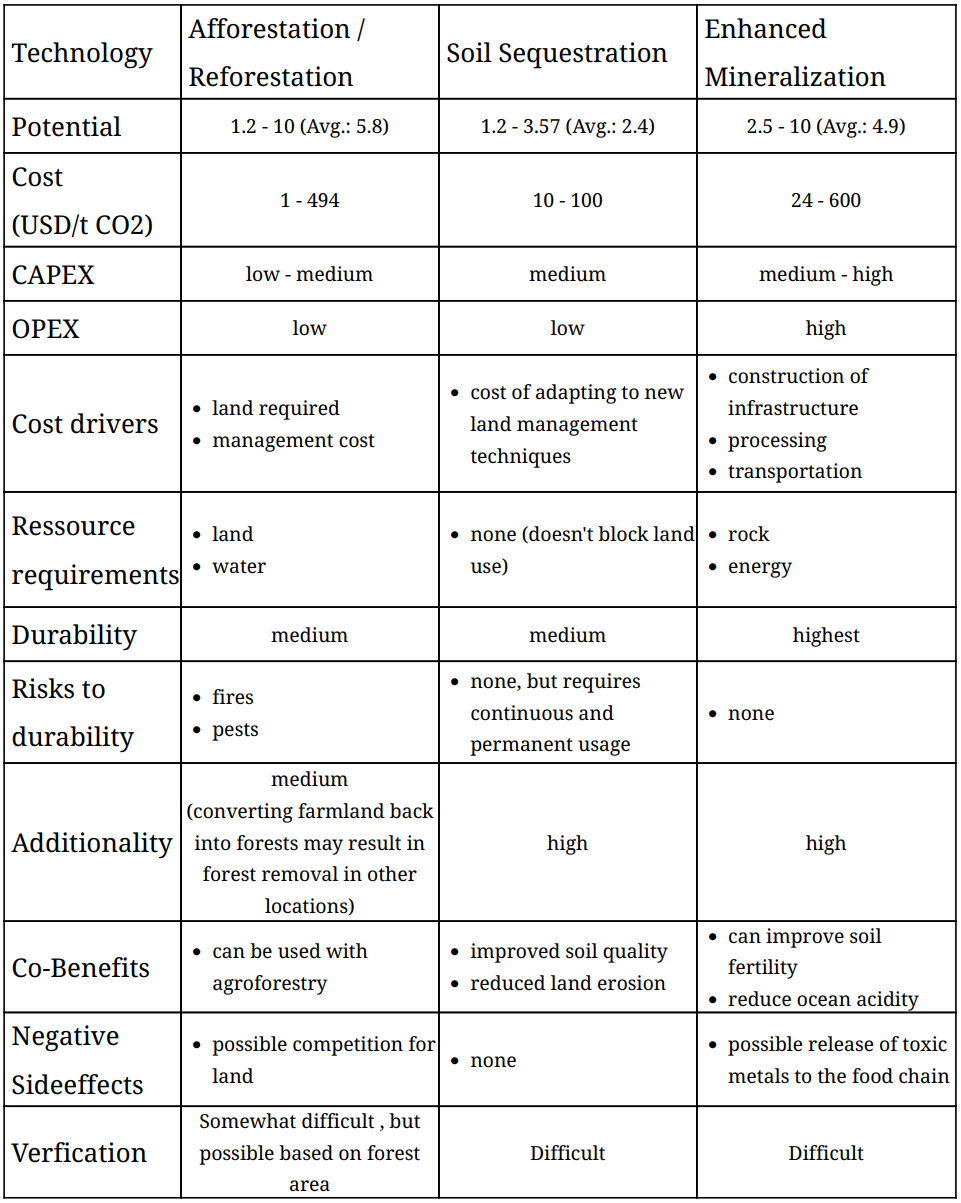
\includegraphics[width=\textwidth]{figures/table1.png}

\appendix
\chapter{Pathway to 1.5 degrees}
\begin{figure}[ht!]
    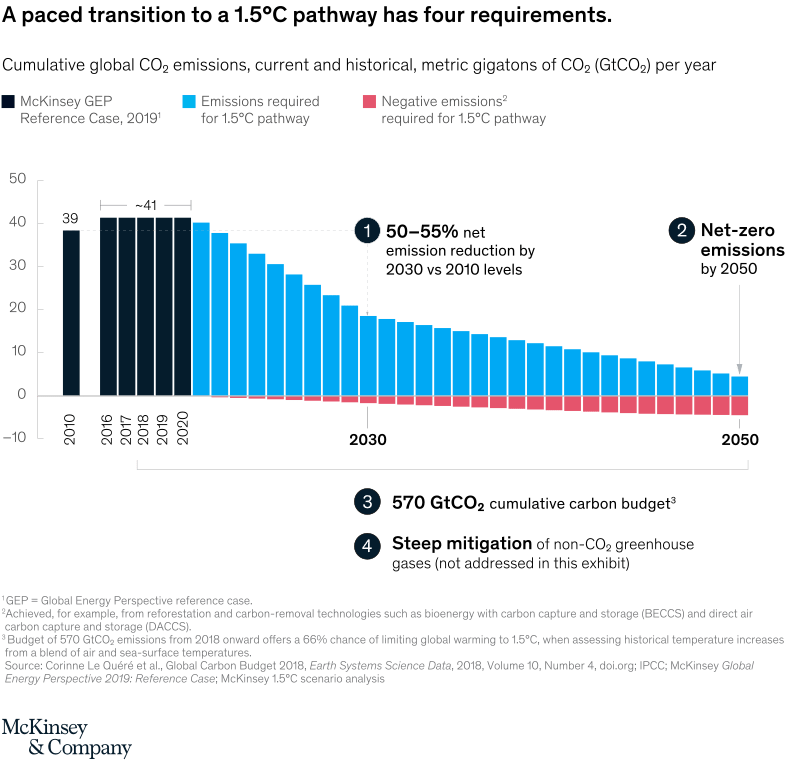
\includegraphics[width=\textwidth]{figures/pathway.png}
    \caption{Projected pathway of carbon emissions reduction required to reach the 1.5-degree goal (Source: McKinsey \& Co., \textit{Climate math: What a 1.5-degree pathway would take})}
\end{figure}
\begin{figure}[ht!]
    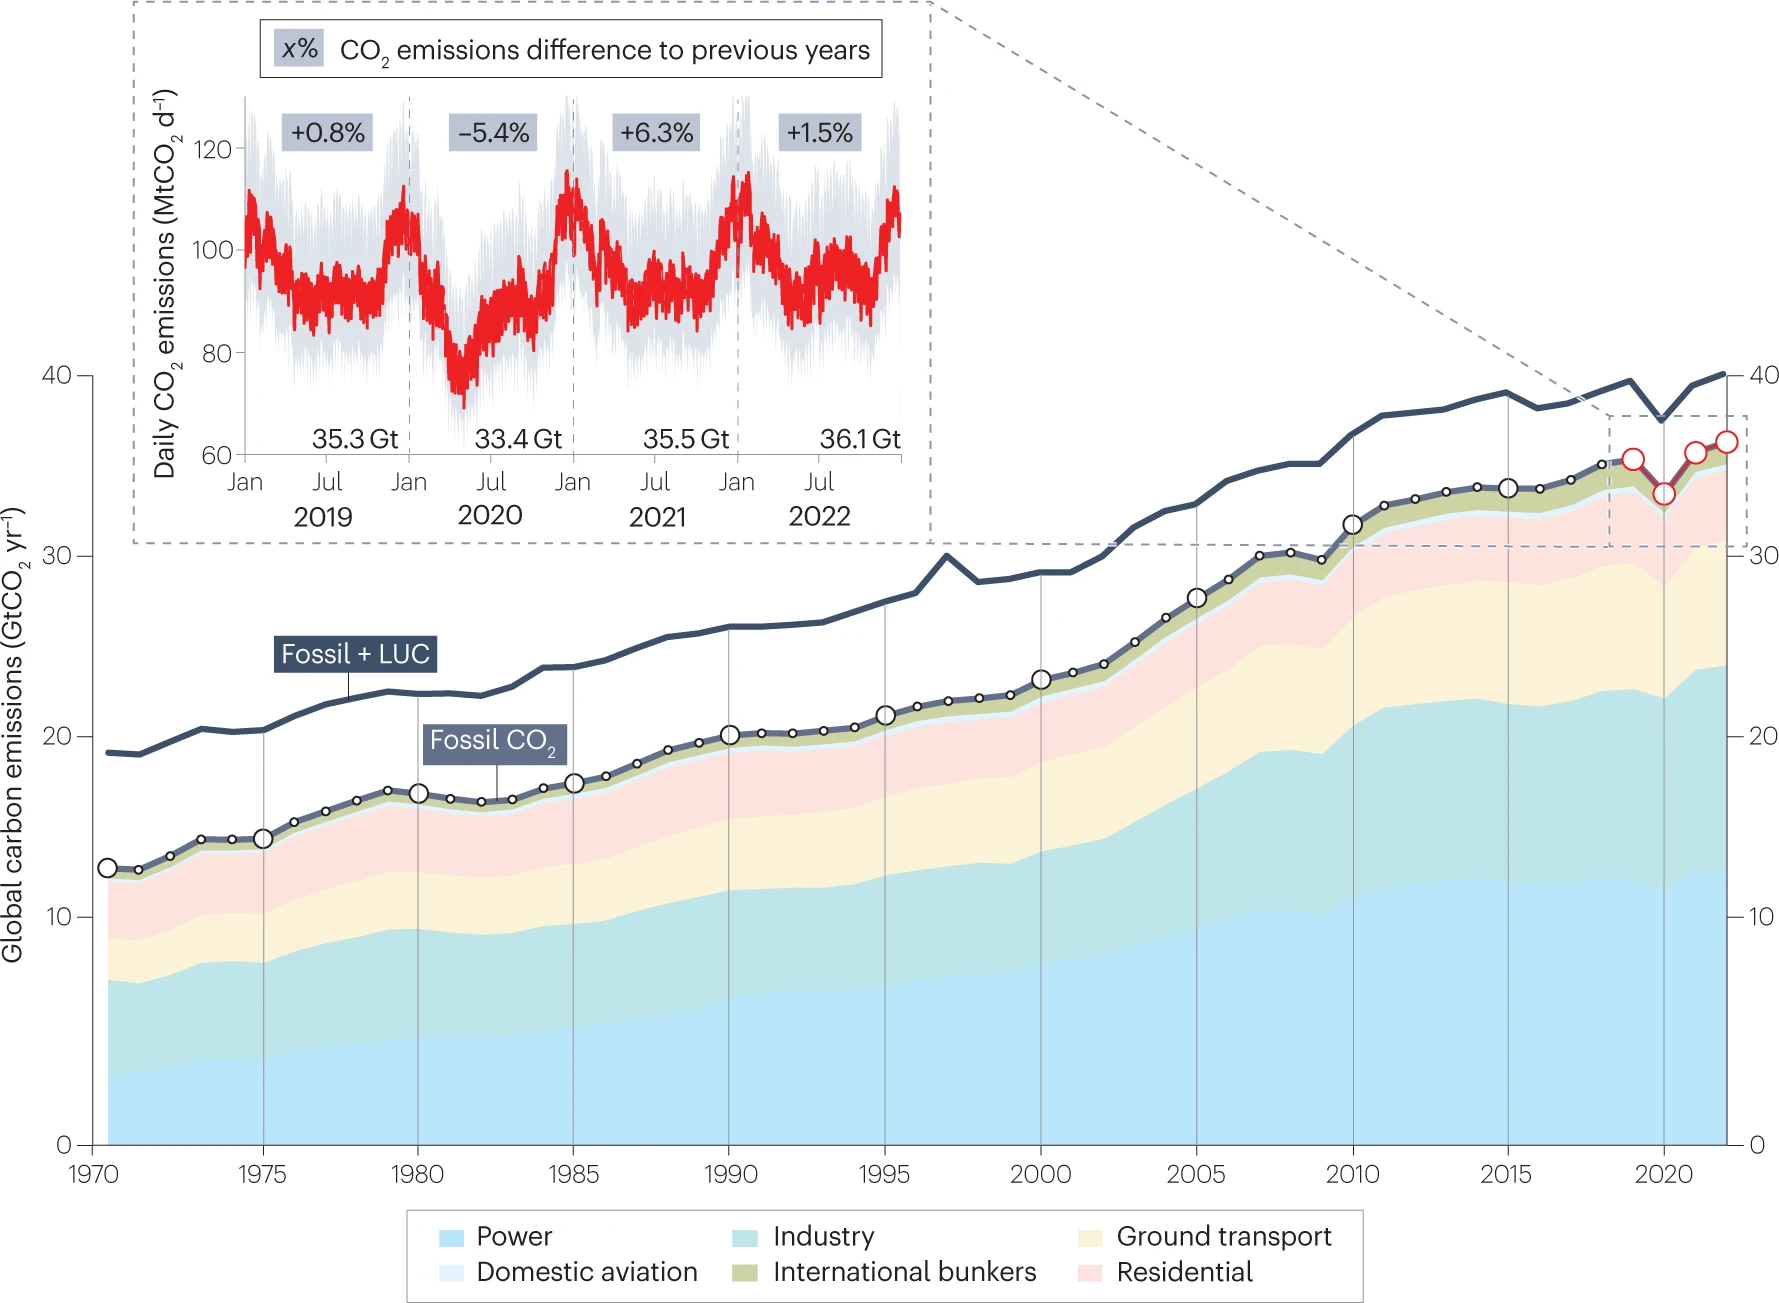
\includegraphics[width=\textwidth]{figures/emissions.png}
    \caption{Actual global carbon dioxide emissions per year from 1900 to 2022 (Source: Liu et al. (2023), \textit{Monitoring global carbon emissions in 2022)}}
\end{figure}

\chapter{Learning effects of DAC}
Learning effects (sometimes called “learning-by-doing”) refer to the phenomenon that individuals or organizations become more efficient or effective at a task over time as they gain experience and knowledge, which can result in significant cost decreases.
This effect was first described by \textcite{Wright1936FactorsAirplanes} in the manufacture of aircraft. He observed that with each doubling of the quantity of aircraft produced, the cost per unit dropped to about 80\% of the previous cost. Since then, learning effects have been observed in a number of manufacturing processes, most prominently in the manufacture of solar photovoltaic modules. Between 2010 and 2020, the cost of solar PV decreased by a factor of five, from approximately 4700 USD/kW to below 900 USD/kW, while the installed capacity increased from 222GW to 1448GW globally. Similar effects, although not of the same magnitude, were observed for wind turbines \parencite{Shrestha2022LearningDeployment}. Mathematically, the experience curve that represents the relationship between the increase in quantity and the reduction in cost is described by \begin{equation} {cost_{new} = cost_{old}*\left( \frac{quantity_{new}}{quantity_{old}} \right)^{-b}} \end{equation} where b is defined as \begin{equation} -b = \frac{\log{PR}}{\log{2}} \end{equation} with PR being the progression ratio, that is, the percentage of the original cost remaining after doubling the quantity \parencite{Fasihi2019Techno-economicPlants}.\\
The literature expects similar learning effects to occur for DAC, based on the similarity of DAC module manufacturing and solar PV module manufacturing. The graph below illustrates possible price decreases, starting with a cost of 600 USD/t CO\textsubscript{2} for an initial 1Mt/y DAC plant. If a 20\% learning rate, that is, an 80\% progress ratio, can be achieved, the cost of DAC would decrease to below 100 USD after the deployment of 260 Mt/y. If an even higher learning rate of 30\%, similar to solar PV, is assumed, this point would be reached at only 33 Mt/y. Using the integral of the experience curve, the necessary investment can be calculated. For a 20\% learning curve, an investment of 37.5 billion USD is required to deploy 260 Mt/y, while for a 30\% learning curve, an investment of 5.5 billion USD would be sufficient to deploy 33 Mt/y.

\begin{figure}[ht!]
    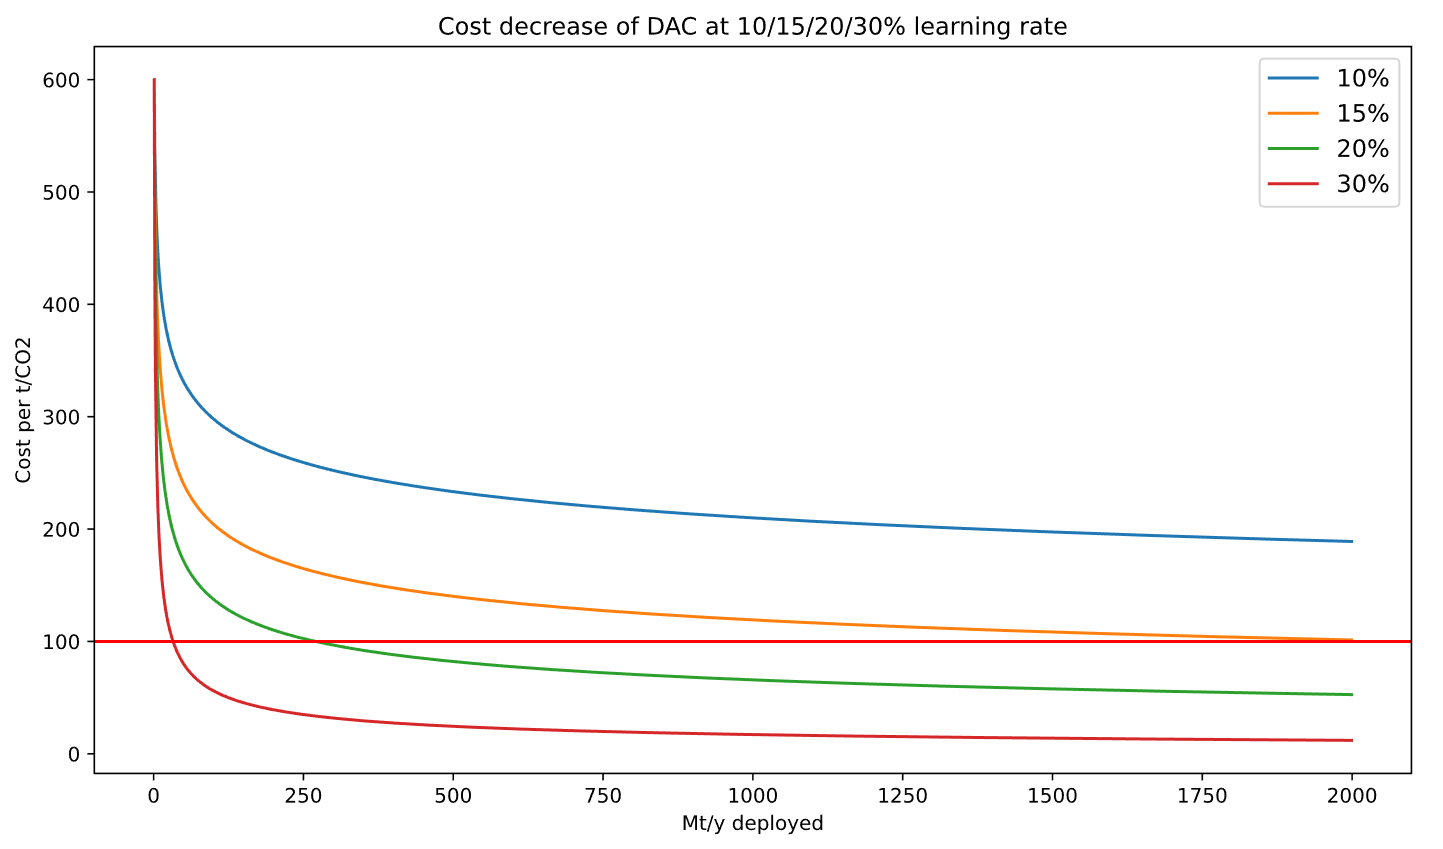
\includegraphics[width=\textwidth]{figures/dac_learning.png}
    \caption{The colored curves show the possible price decreases at different learning rates. The red horizontal line represents the 100 USD/t threshold that must be reached to make DAC economically viable.}
\end{figure}
\newpage
\noindent From this figure it can be concluded that the learning rate will have a significant impact on the future of DAC technology. If a high learning rate is realized, DAC will become relatively cheap rather quickly as commercial deployment progresses. However, if only a low learning rate is observed, DAC may stay prohibitively expensive for the foreseeable future.

\chapter{Overview of potential and cost estimates}
 \mbox{} \begin{center}
    \begin{sideways}%[htbp]
    \captionsetup{margin=0cm}
         \begin{minipage}{1.2\linewidth}
            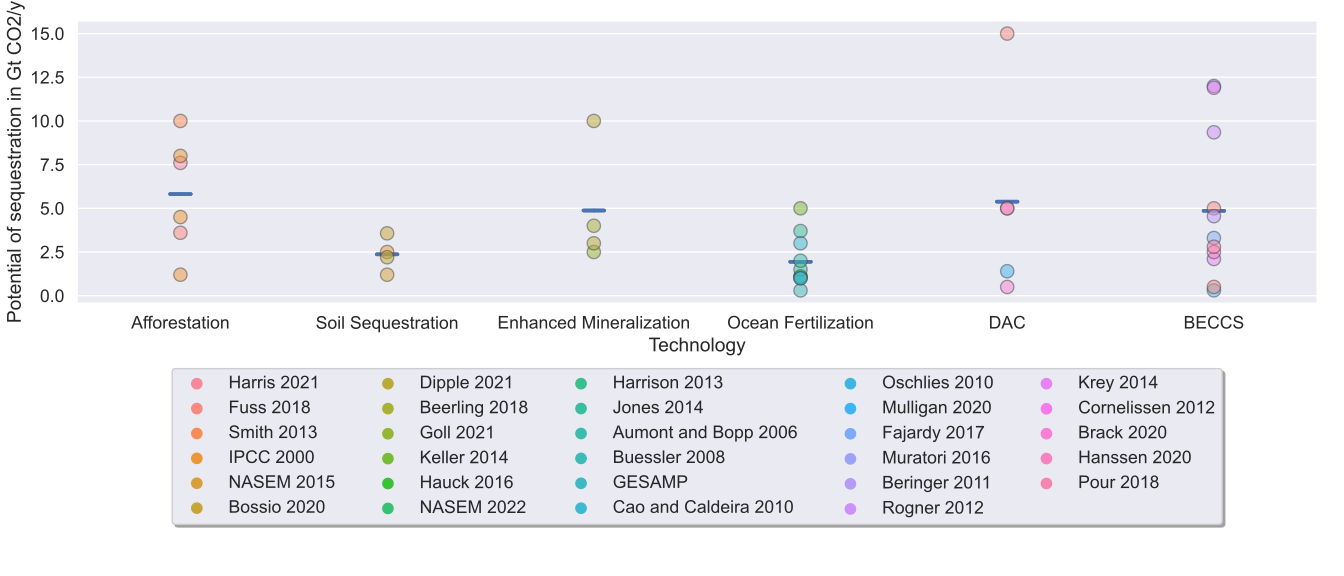
\includegraphics[width=550pt, keepaspectratio]{figures/potential.png}
            \captionof{figure}{Overview of the potential of CDR approaches mentioned in literature. The blue lines represent the average values.}
         \vspace{0.2cm}
         \label{fig:xx}
         \end{minipage}
    \end{sideways}
    \end{center}

\begin{sidewaysfigure}
\captionsetup{margin=3.5cm}
    \centering
    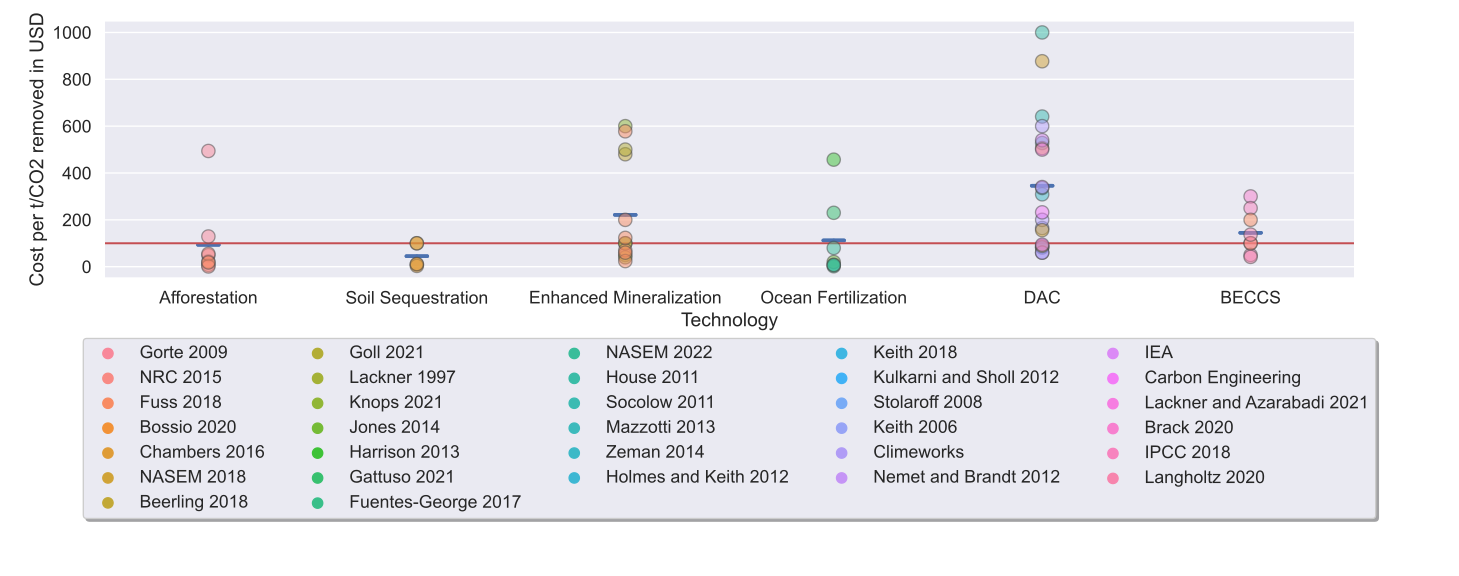
\includegraphics[width=600pt]{figures/cost.png}
    \caption{Overview of the cost of CDR approaches mentioned in literature. The blue lines represent the average values. The red line represents the 100 USD threshold.}
    \label{fig:awesome_image}
\end{sidewaysfigure}

\nocite{House2011EconomicAir, Aumont2006GlobalizingStudies, Buesseler2008OceanUncertainty, Cao2010ImportanceChange, Oschlies2010ClimateApprentice, Beringer2011BioenergyConstraints, Rogner2012EnergyPotentials, Krey2014GlobalReview, Cornelissen2012TheSystem}
\nocite{Cornelissen2012TheSystem, Mazzotti2013DirectContactor, Socolow2011DirectAffairs, Zeman2014ReducingCO2, Nemet2011WillingnessCapture, Kulkarni2012AnalysisAir, Stolaroff2008CarbonSpray}
\nocite{McKinsey2020ClimateTake, Liu2023Monitoring2022}

\printbibliography

\newpage \noindent
{\large \textbf{Statutory Declaration}}\\
\\I hereby guarantee that the present paper is my own and that I have properly acknowledged any help or support received from other individuals. Furthermore, I declare that neither this work nor parts of it have been submitted by myself or others to another university as part of a formal degree requirement. All intellectual property of others is clearly cited as such.\\
\\All secondary literature and other sources are certified and listed in the bibliography. The same applies for graphic illustrations, pictures and all internet sources.\\
\\I agree that my work may be electronically saved and sent anonymized to be checked for plagiarism. I am aware that this paper cannot be graded if this declaration is not signed.\\
\\Mannheim, …………………… ……………………………………
\end{document}
